\chapter{QDPT vs DPT with increasing coupling modes}

\begin{figure}[h!]
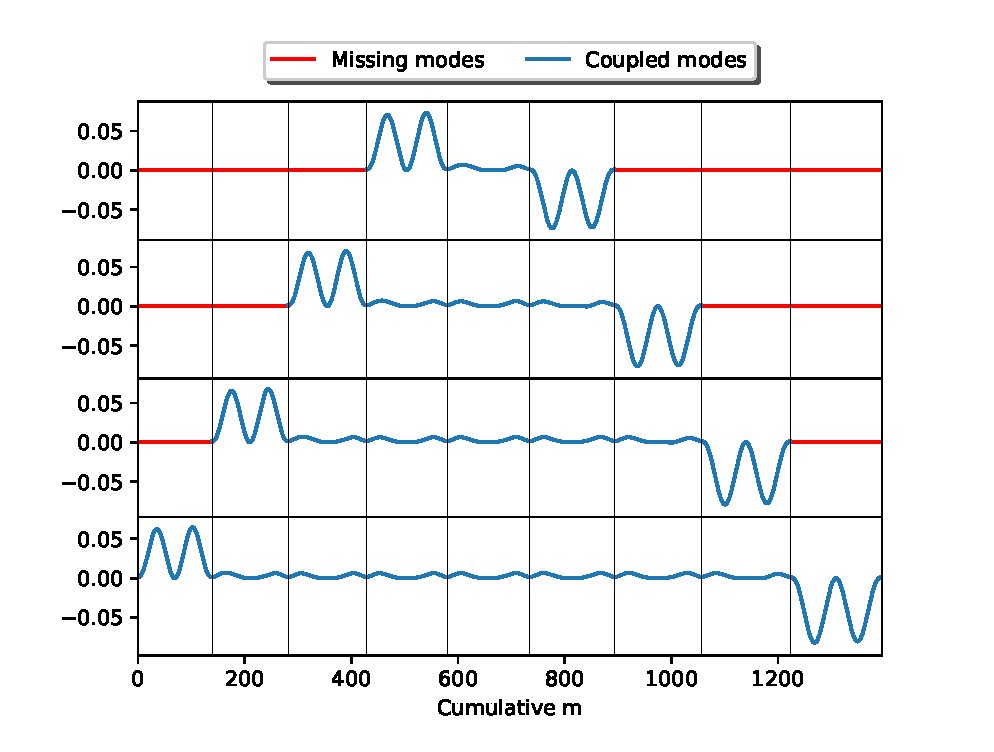
\includegraphics[scale=0.9, center]{Chapter4/figs/qdpt_err}
\caption{(QDPT - DPT) deviation with differing number of neighbouring modes being allowed to couple. From top, $\mode{0}{77}$ is made to couple with two, four, six, and eight closest $\Delta l=2$ neighbours (by frequency) as listed in table \ref{tab:mode_list}. The trend shows large deviations from DPT frequencies in modes placed at either extreme regardless of how many modes couple while QDPT-DPT departure in the inner modes stay the same. This hints at QDPT frequencies obtained for the extremal modes being artefacts of the calculation and hence being unreliable.}
\label{fig:DPT_err} 
\end{figure}